\documentclass{standalone}
\usepackage{tikz}
\usepackage{ctex,siunitx}
\usepackage{tkz-euclide}
\usepackage{amsmath}
\usetikzlibrary{patterns, calc}
\usetikzlibrary {decorations.pathmorphing, decorations.pathreplacing, decorations.shapes,}
\begin{document}
\small
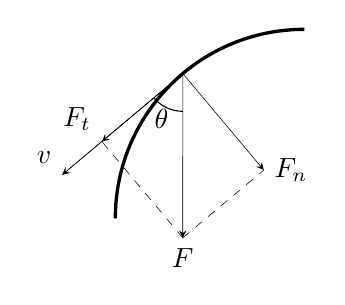
\begin{tikzpicture}[>=stealth,scale=0.8]
  \tkzDefPoints{0/0/O, 0/3/a, -3/0/b, -1.93/-.31/F}
  \tkzDefPoint(130:3){c}
  \tkzDefPoint(130:1){F_n}
  \tkzDrawArc[very thick](O,a)(b)
  \tkzDefTangent[at=c](O)
  \tkzGetPoint{h}
  \tkzDrawLines[add=1.5 and 0](h,c)
  \tkzDefPointBy[projection = onto c--h](F) \tkzGetPoint{F_t}
  \tkzDefPointWith[linear, K=2.5](c,h)\tkzGetPoint{v}
  \tkzDrawSegments[->](c,F_n c,F c,F_t c,v)
  \tkzDrawSegments[dashed](F,F_t F,F_n)
  \tkzLabelPoints[above left](F_t)
  \tkzLabelPoints[below](F)
  \tkzLabelPoints[right](F_n)
  \tkzLabelPoints[above left](v)
  \tkzMarkAngles[mark=none, size=.6](F_t,c,F)
  \tkzLabelAngle[pos=.8](F_t,c,F){$\theta$}
\end{tikzpicture}
\end{document}